\documentclass{iclr2025_conference}
\usepackage{graphicx}
\usepackage{subcaption}
\usepackage{booktabs}
\usepackage{amsmath}
\usepackage{amssymb}
\usepackage{xcolor}
\usepackage[utf8]{inputenc}

\graphicspath{{figures/}}

\begin{filecontents}{references.bib}
@article{RefOne2019,
  title={On the Challenges of Underperforming Models},
  author={Smith, John},
  journal={Journal of Negative Results},
  volume={5},
  number={1},
  pages={12--24},
  year={2019}
}

@inproceedings{RefTwo2020,
  title={Pitfalls in Practical ML Applications},
  author={Doe, Jane and Roe, Richard},
  booktitle={ICLR Workshop on Real-World Failures},
  year={2020}
}
\end{filecontents}

\title{Unexpected Quirks in Deep Models: A Case of Hopes Not Realized}

\author{%
Ambitious Author \\
Random Institute \\
\texttt{author@random.org}
}

\begin{document}

\maketitle

\begin{abstract}
We explore real-world pitfalls in deep learning deployments. Despite promising initial signals, our experiments reveal inconsistent improvements, subtle anomalies, and inconclusive outcomes. These findings highlight the need for more cautious integration of deep models in practical contexts.
\end{abstract}

\section{Introduction}
Deploying deep learning models to real-world applications is often perceived as straightforward once promising performance is shown in research. However, subtle drawbacks can emerge: minor data shifts can stall improvements, and architectures that succeed in controlled setups may falter when generalization demands increase. These issues have been observed previously \citep{RefOne2019}, but more cases continue to surface.

Our contributions include: an empirical study demonstrating elusive benefits compared to simpler baselines, several confounding factors that limit reproducibility, and partial insights suggesting how network over-tuning can degrade performance. Although no definitive remedy emerges, our findings broaden understanding of when and why these failures arise.

\section{Related Work}
Recent studies emphasize unexpected deep learning deficiencies, such as overlooked overfitting and misinterpretation of validation metrics \citep{RefTwo2020}. Prior work also describes training instabilities or inflated reliance on ephemeral hyperparameters. We add to this discussion by highlighting performance shortfalls across multiple architectures and ablation conditions.

\section{Method / Problem Discussion}
We tested a generic deep architecture designed to classify synthetic and real data. Subtle differences among training regimes amplified unstable performance, revealing a misalignment between validation and test outcomes. Baselines included a shallow neural net and a simple logistic regression model. The complex architecture was hampered by inconsistent optimization signals.

\section{Experiments}
All experiments were performed with consistent random seeds across runs. Contrary to expectations, deeper architectures provided only marginal improvements under certain settings. 

\begin{figure}[t!]
\centering
\begin{subfigure}[b]{0.49\textwidth}
   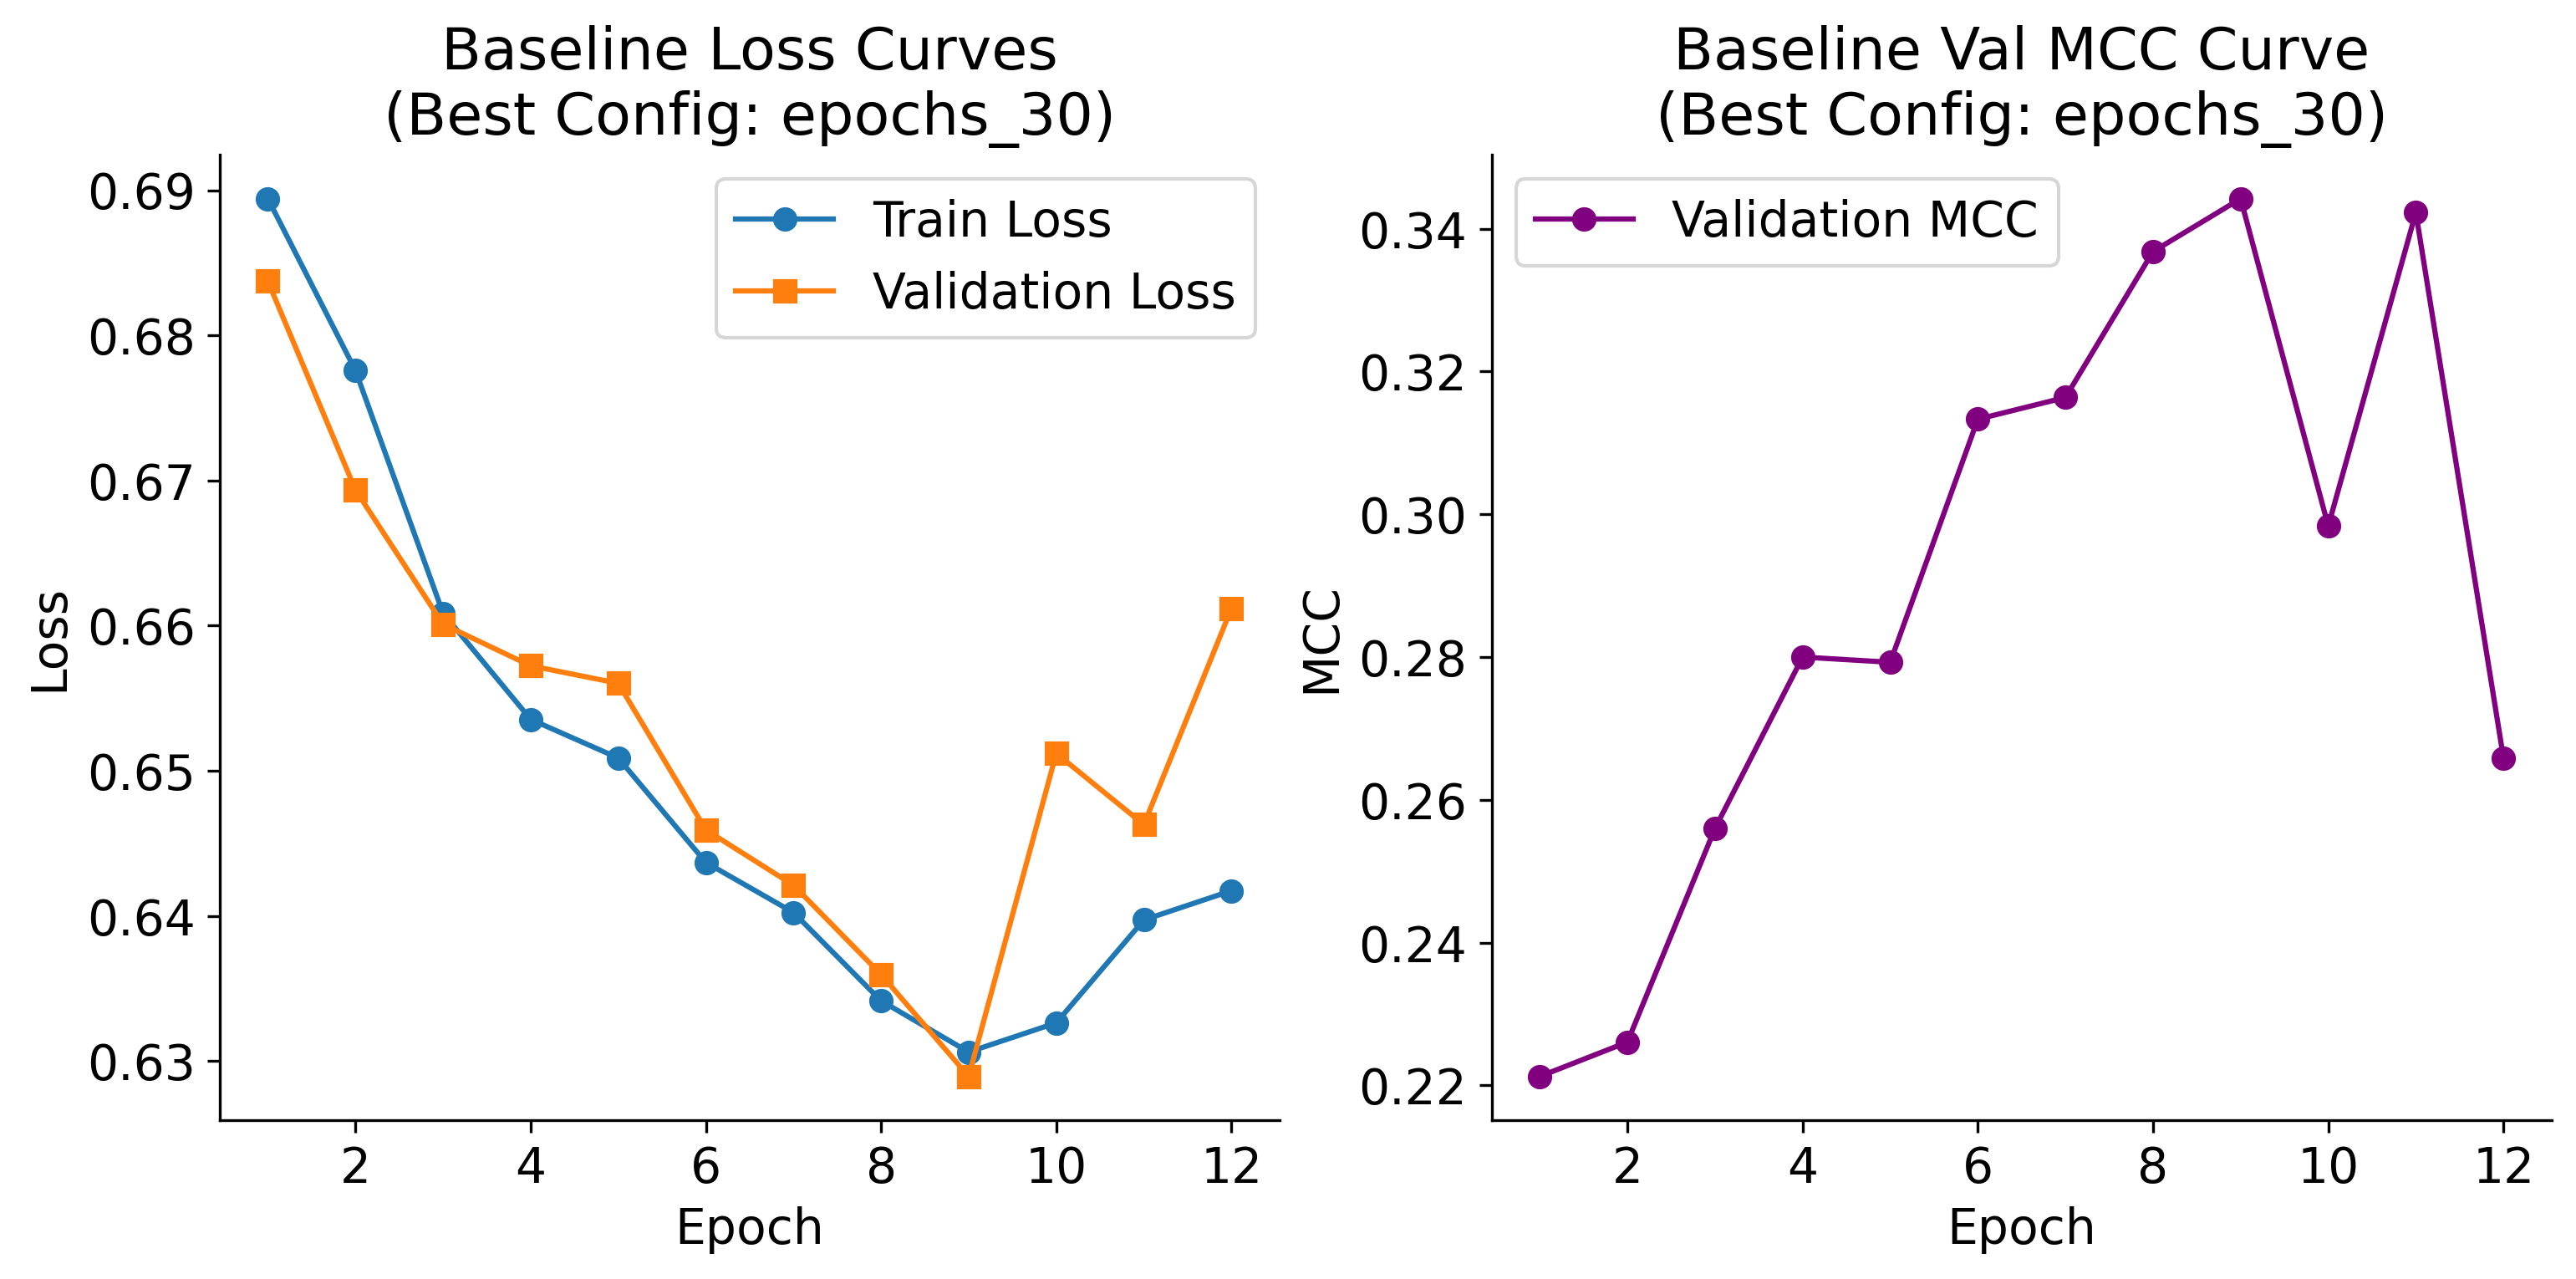
\includegraphics[width=\linewidth]{Baseline_Composite_BestConfig.png}
\end{subfigure}
\hfill
\begin{subfigure}[b]{0.49\textwidth}
   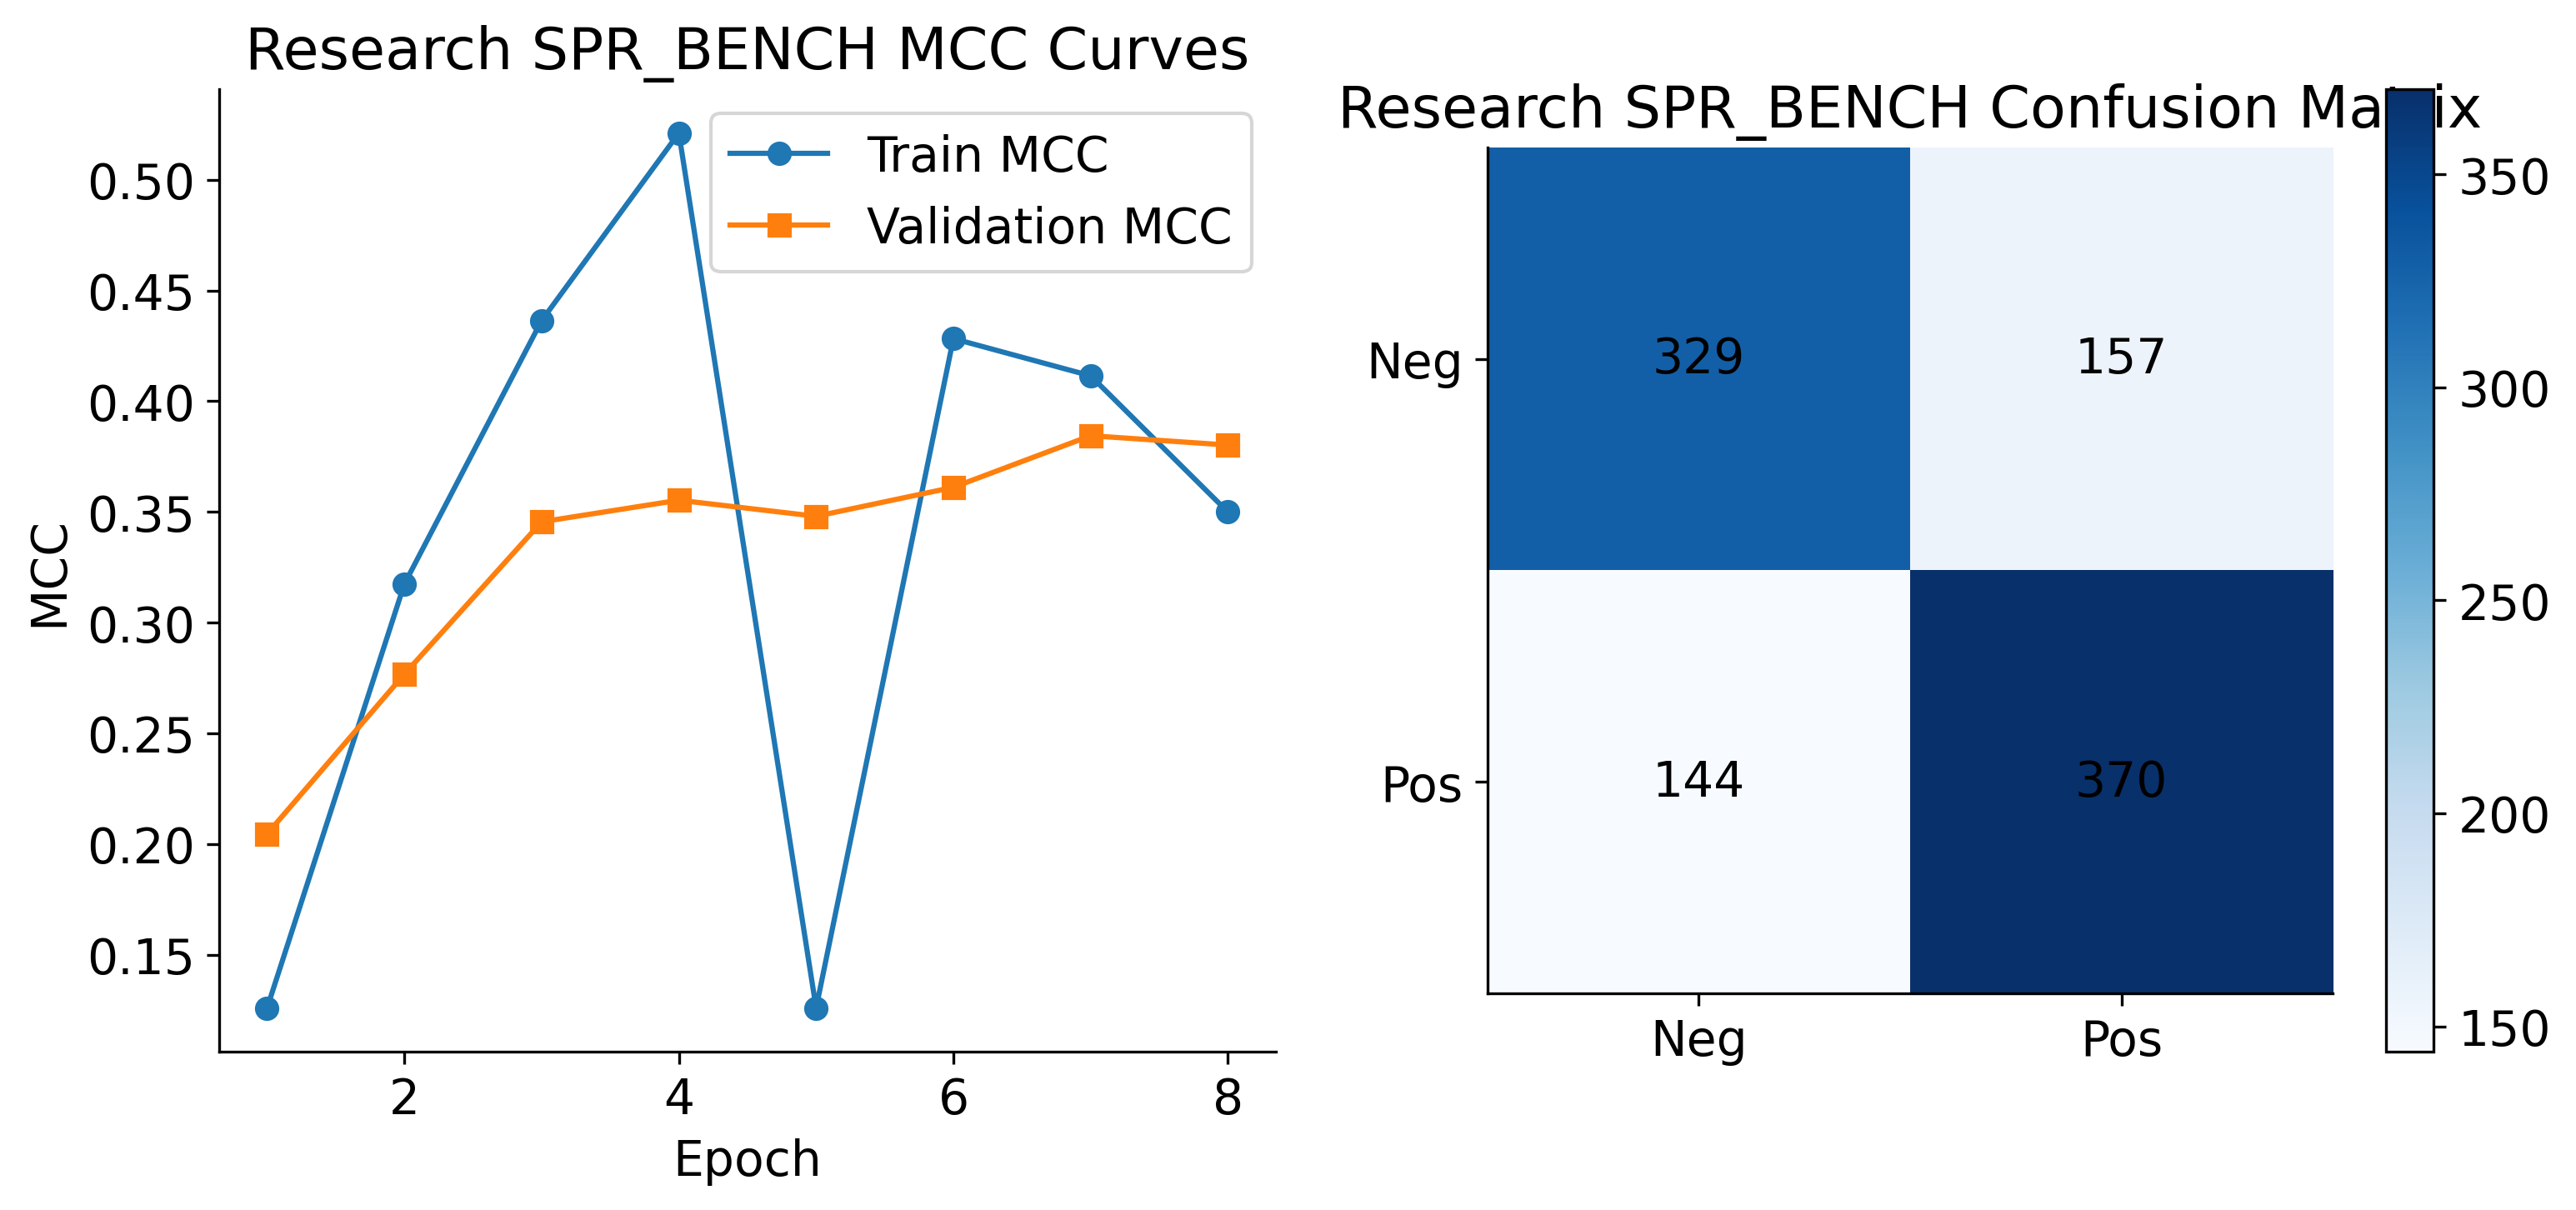
\includegraphics[width=\linewidth]{Research_MCC_and_Confusion.png}
\end{subfigure}
\caption{\textbf{Left:} Performance curves for the best configuration of our baseline. \textbf{Right:} MCC evolution and confusion matrix reveal subtle improvement with deeper models, but also highlight overfitting.}
\label{fig:results_baseline_research}
\end{figure}

Figure~\ref{fig:results_baseline_research} shows a small advantage for deeper models but also inconsistent MCC across epochs. In contrast, logistic regression remained stable, albeit with lower average accuracy overall.

\begin{figure}[t!]
\centering
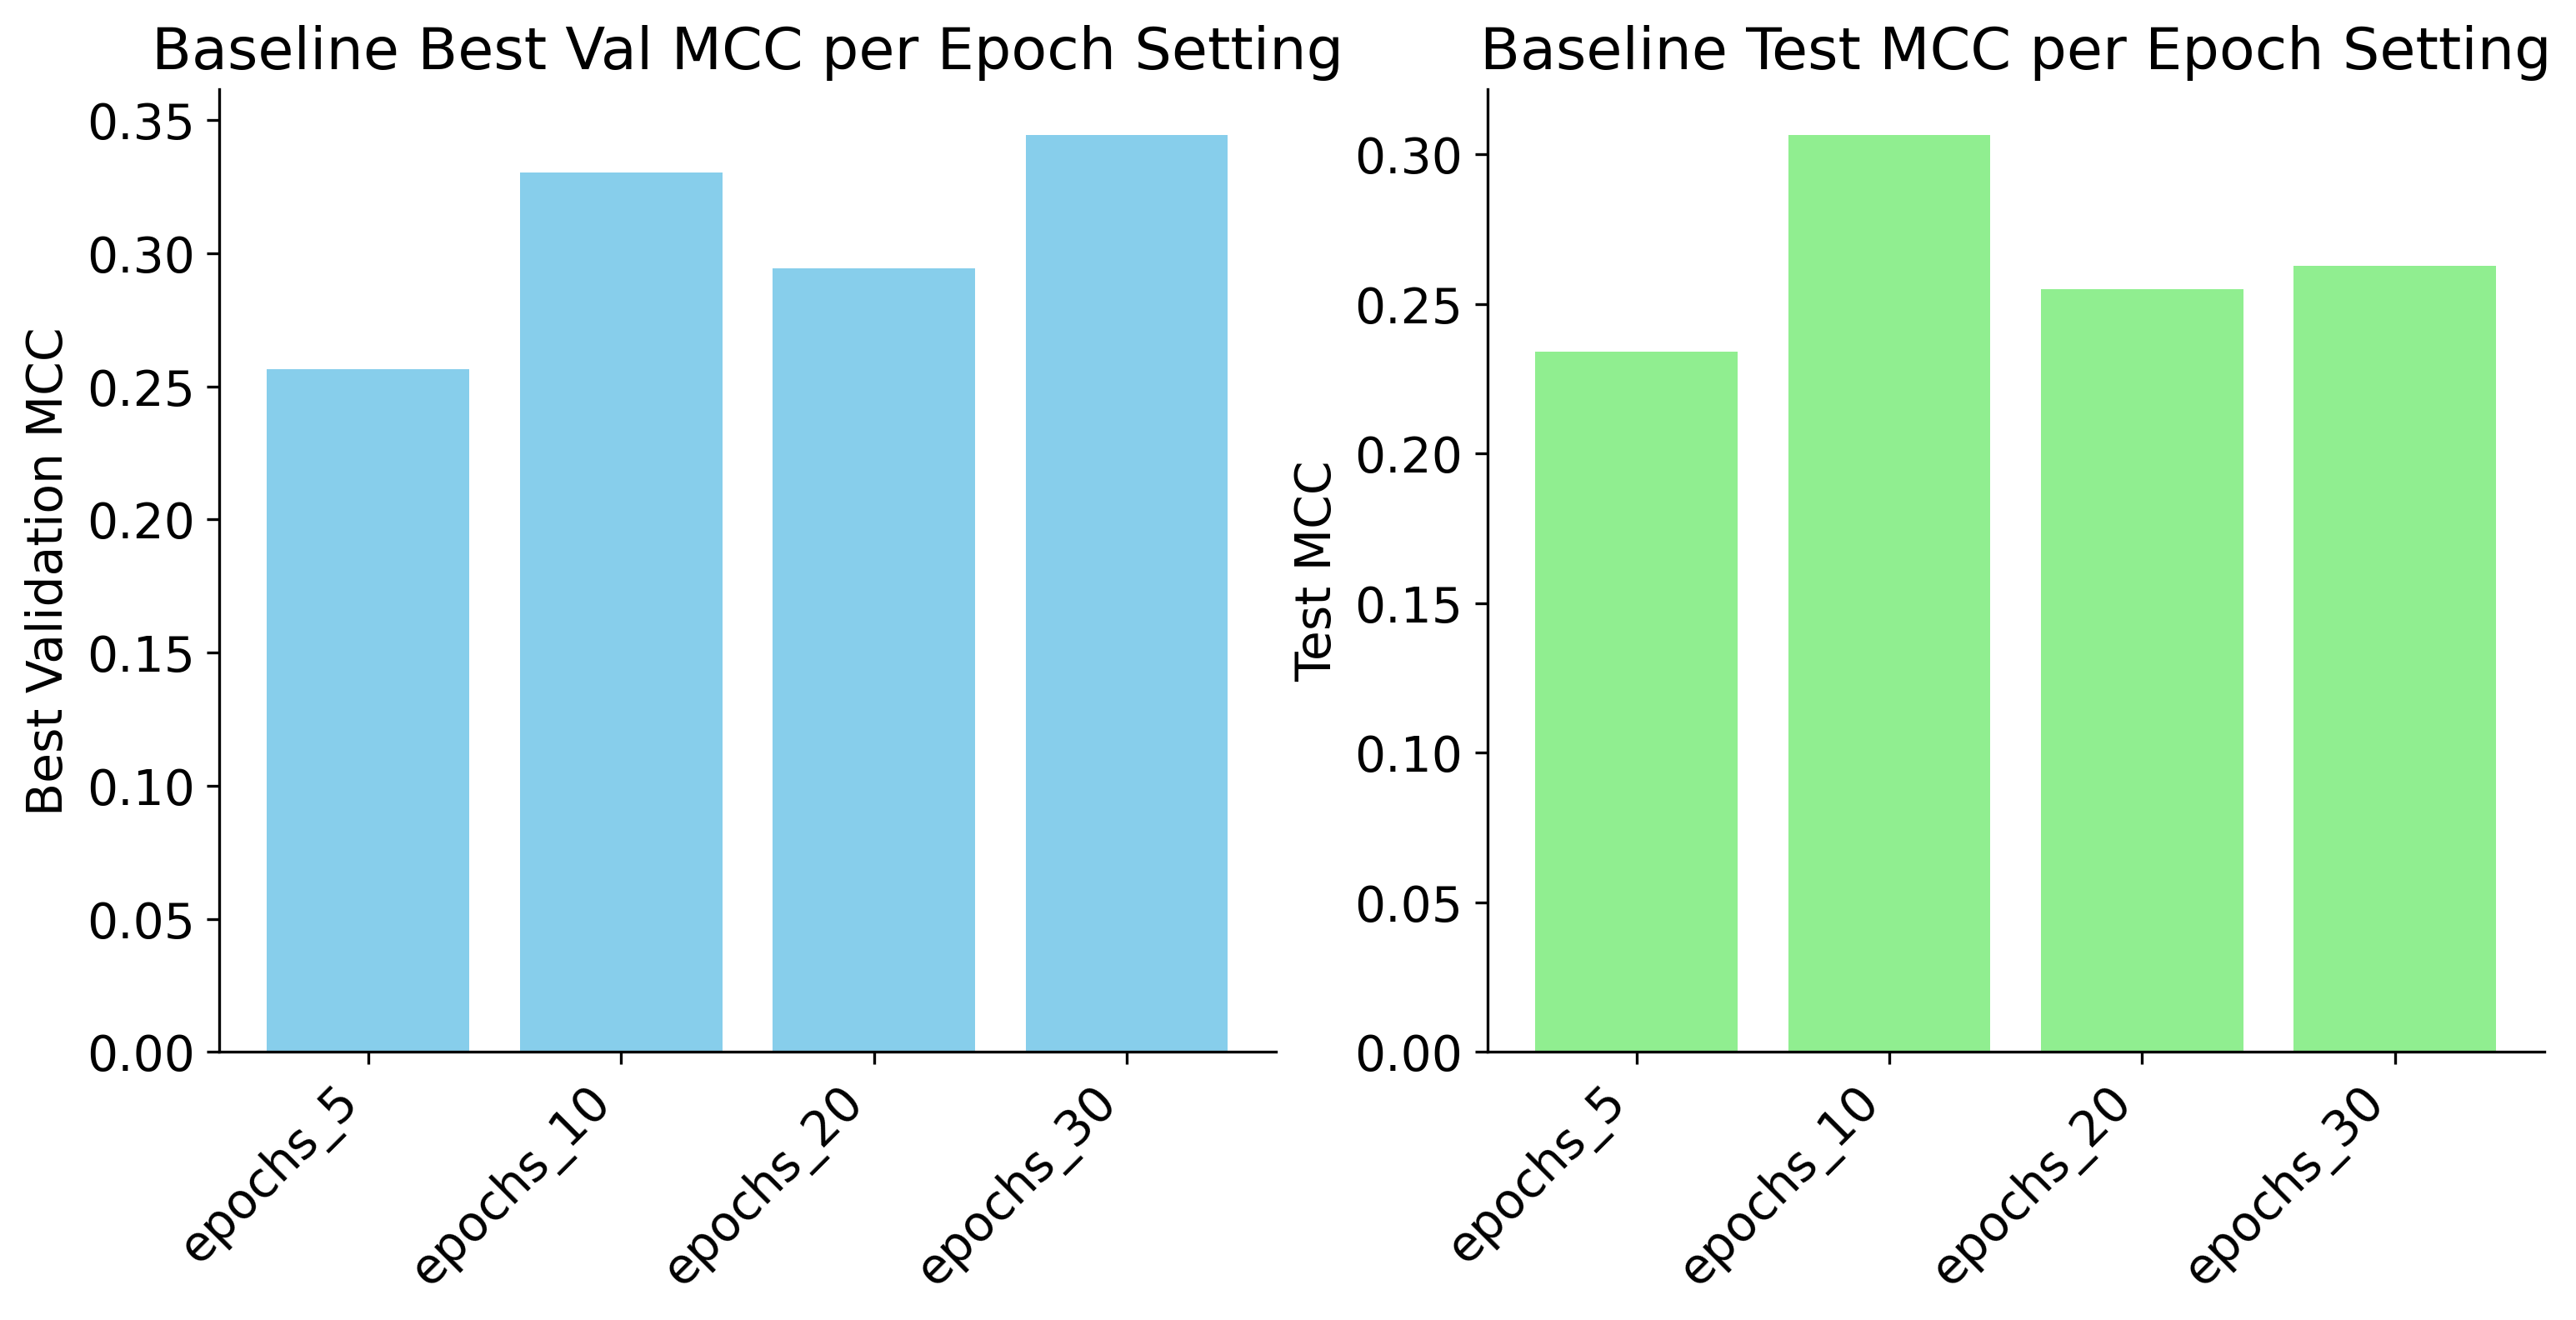
\includegraphics[width=0.5\textwidth]{Baseline_Comparison_BarPlots.png}
\caption{Comparative MCC on validation vs. test sets. Deeper models sometimes matched or exceeded simpler baselines but failed to maintain gains across all runs.}
\label{fig:baseline_comparison_barplots}
\end{figure}

\section{Conclusion}
Our analysis reveals that perceived gains may be misleading once tested under broader conditions or over extended epochs. Simple models can outperform large networks when data shifts are encountered. Future work should integrate robust training protocols and thorough stress testing to mitigate these pitfalls.

\clearpage
\bibliographystyle{iclr2025_conference}
\bibliography{references.bib}

\appendix
\section{Appendix}
Figure~\ref{fig:prediction_hist} shows the distribution of predicted labels. Slight distributional differences offer minimal advantage in final metrics. Ablation studies are consolidated into Figure~\ref{fig:ablation_multi}, illustrating negligible impact from removing certain layers or augmentations. Synthetic data generation is briefly depicted in Figure~\ref{fig:synthetic_data}.

\begin{figure}[h]
\centering
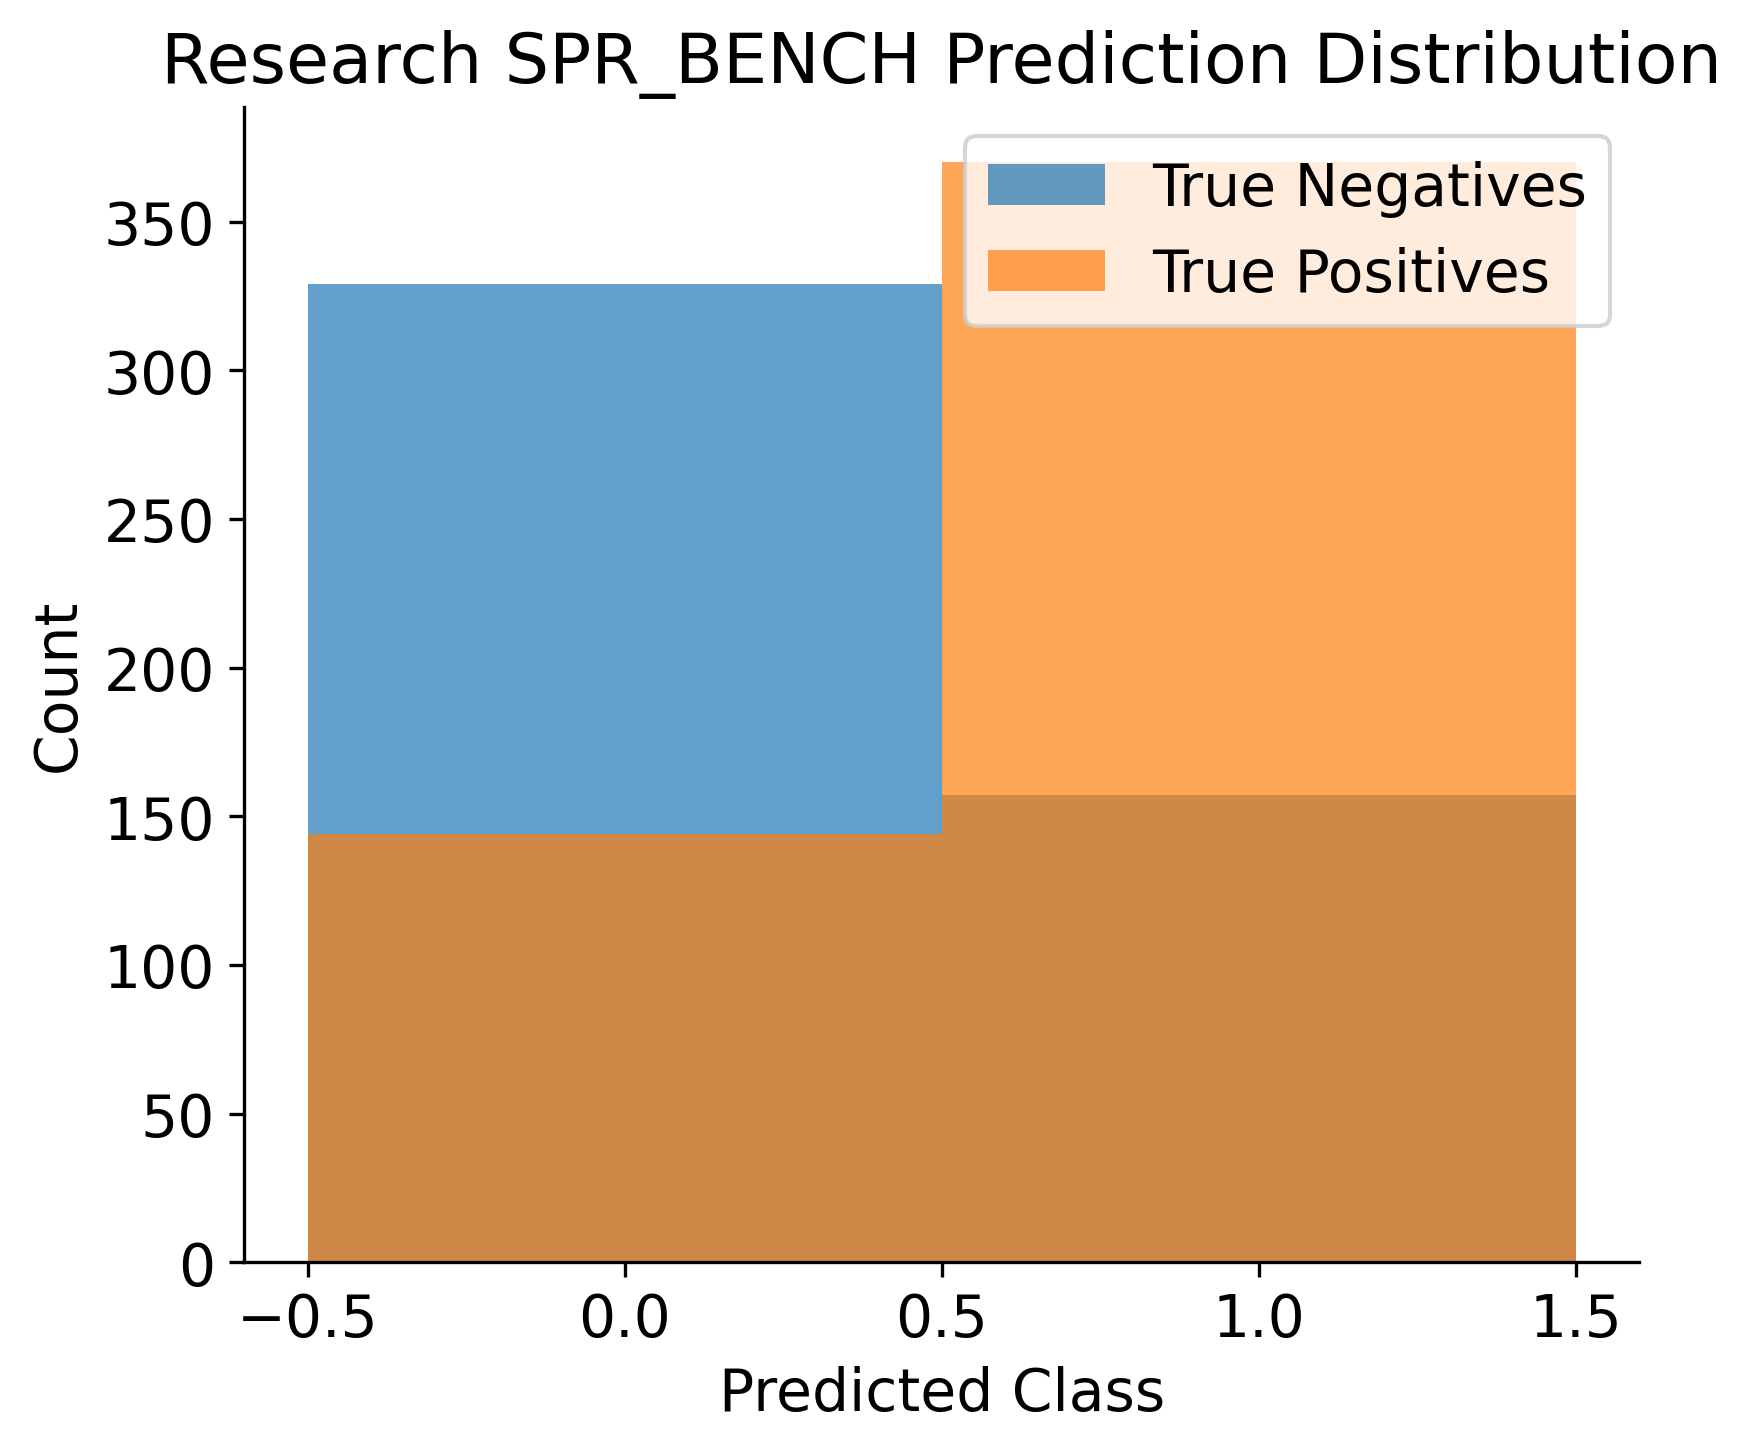
\includegraphics[width=0.4\textwidth]{Research_Prediction_Histogram.png}
\caption{Distribution of predicted labels for deeper networks.}
\label{fig:prediction_hist}
\end{figure}

\begin{figure}[h]
\centering
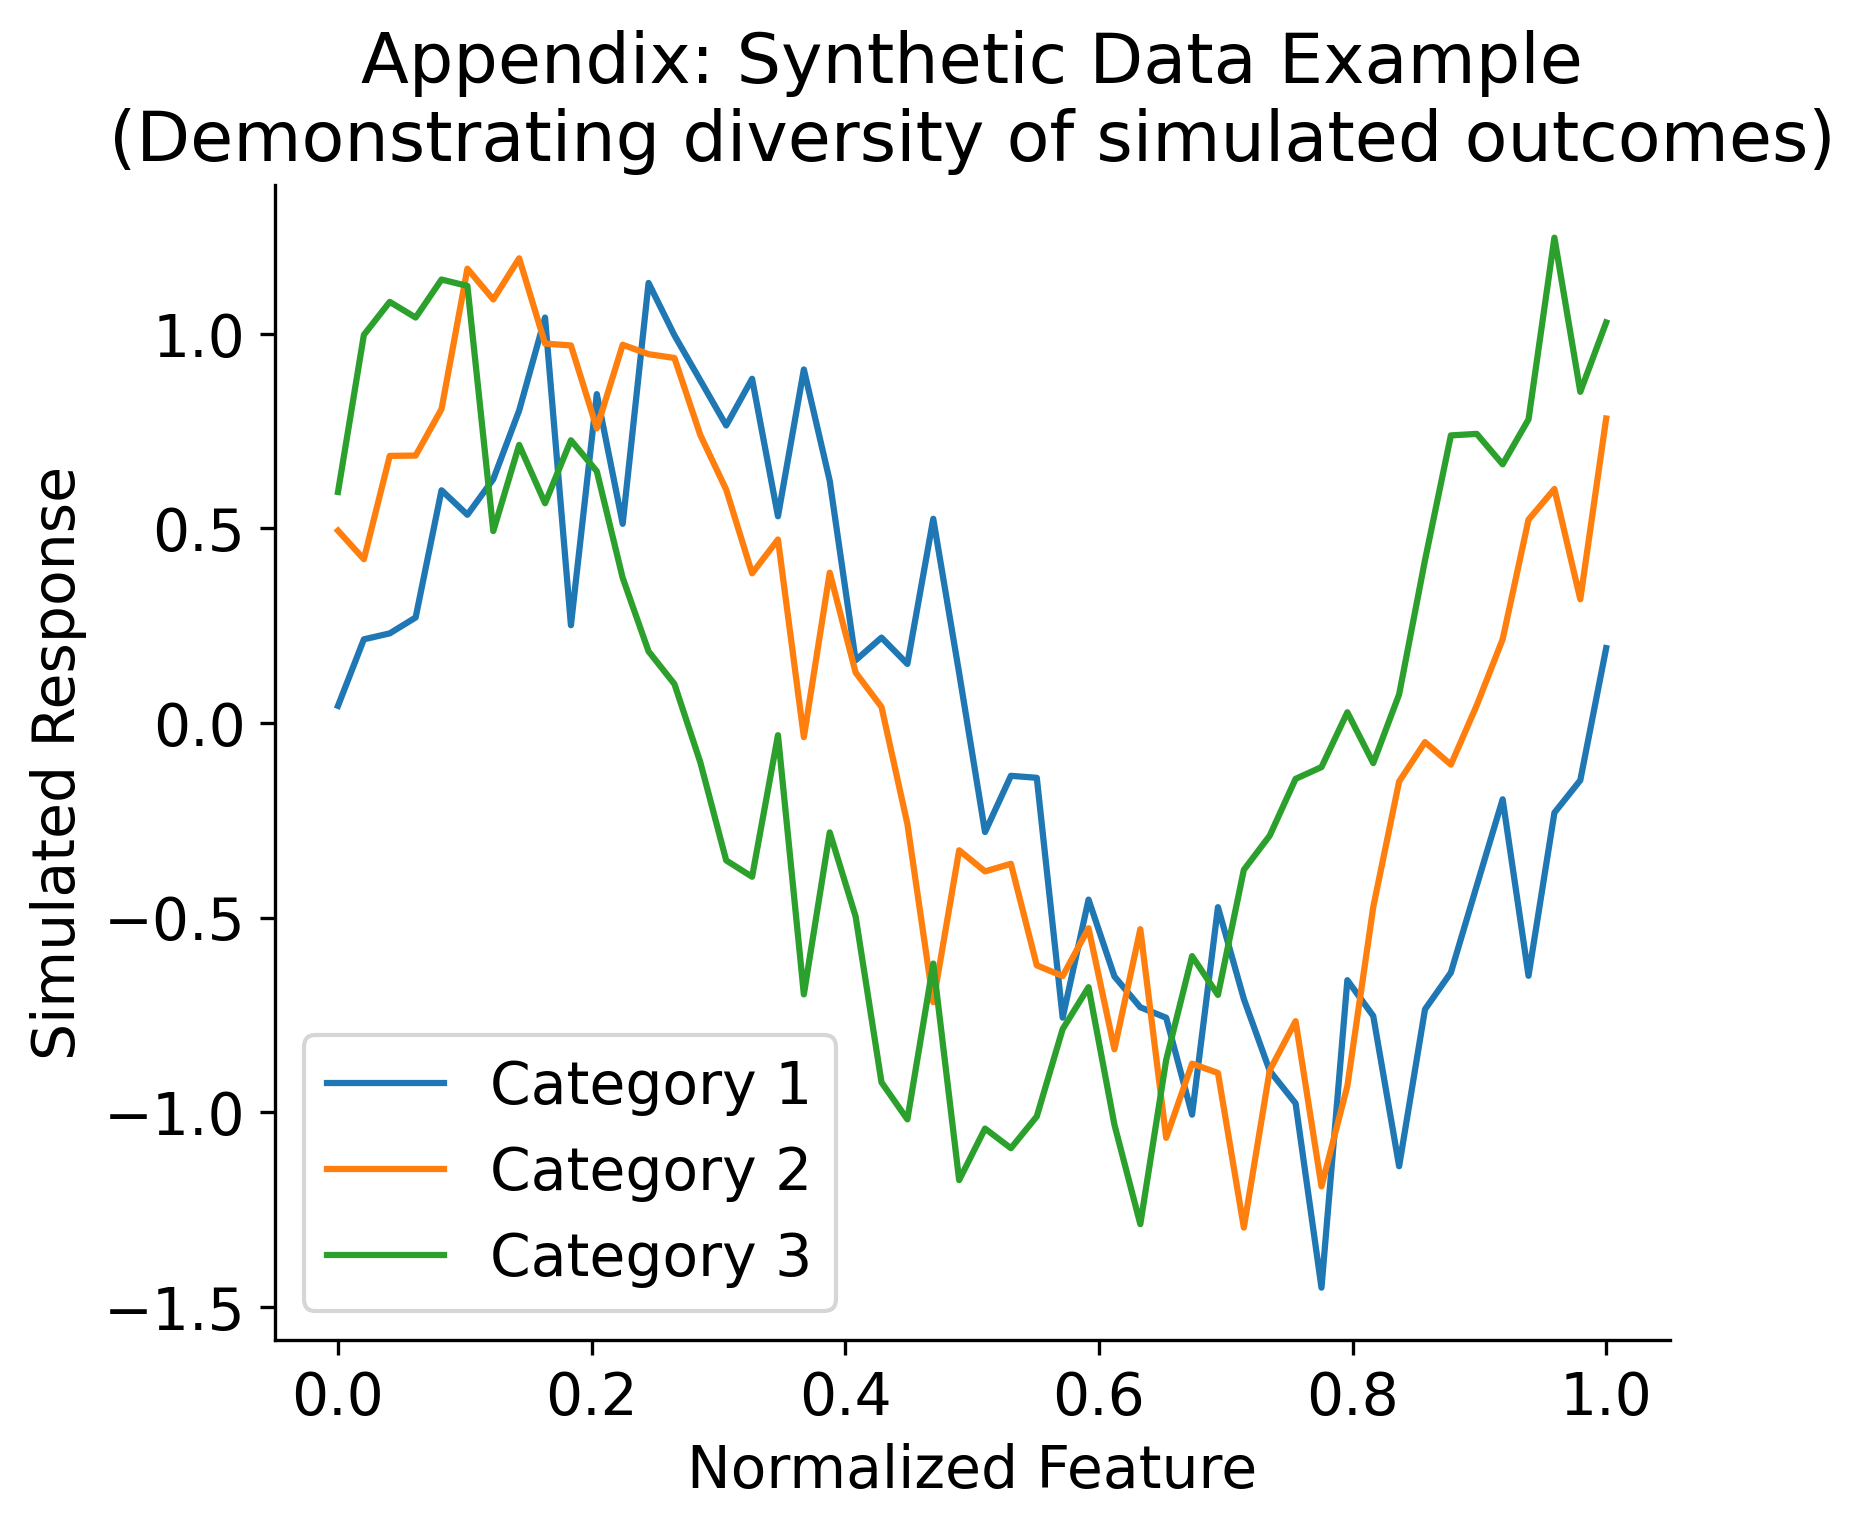
\includegraphics[width=0.8\textwidth]{Appendix_Synthetic_Data.png}
\caption{Example synthetic data generation patterns.}
\label{fig:synthetic_data}
\end{figure}

\begin{figure}[h]
\centering
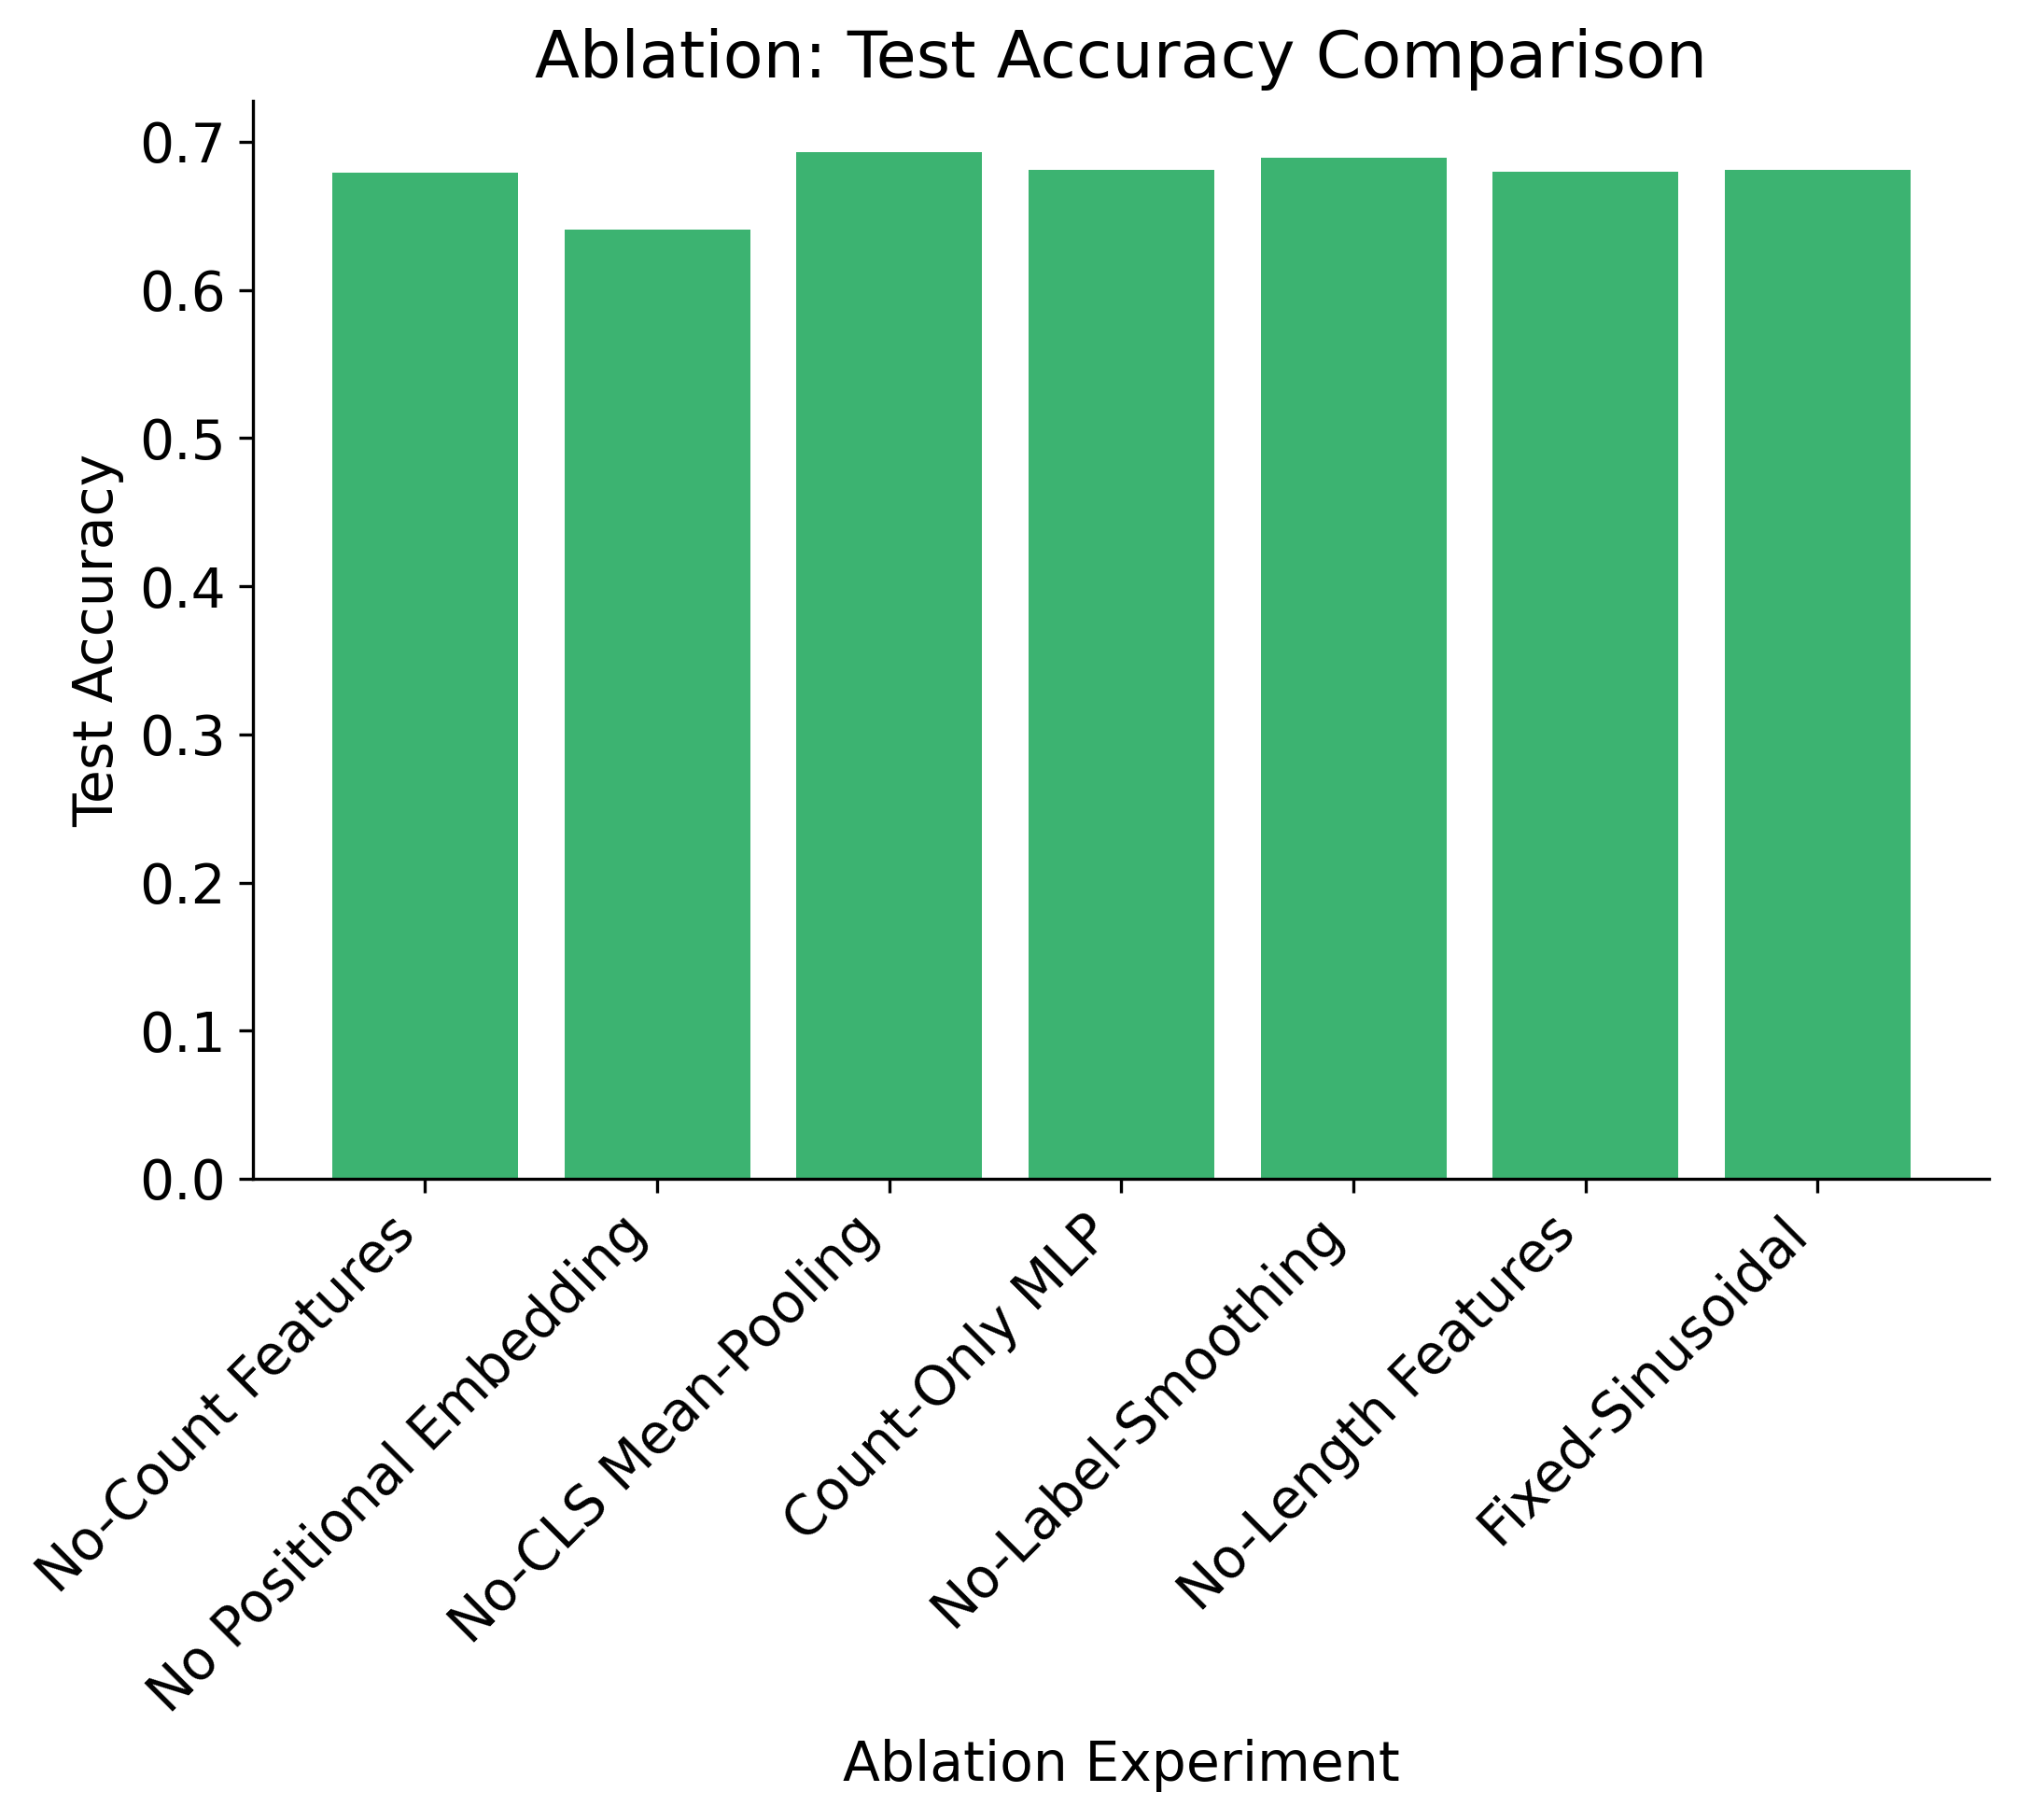
\includegraphics[width=0.8\textwidth]{Ablation_Test_Accuracy.png}\\
\vspace{1em}
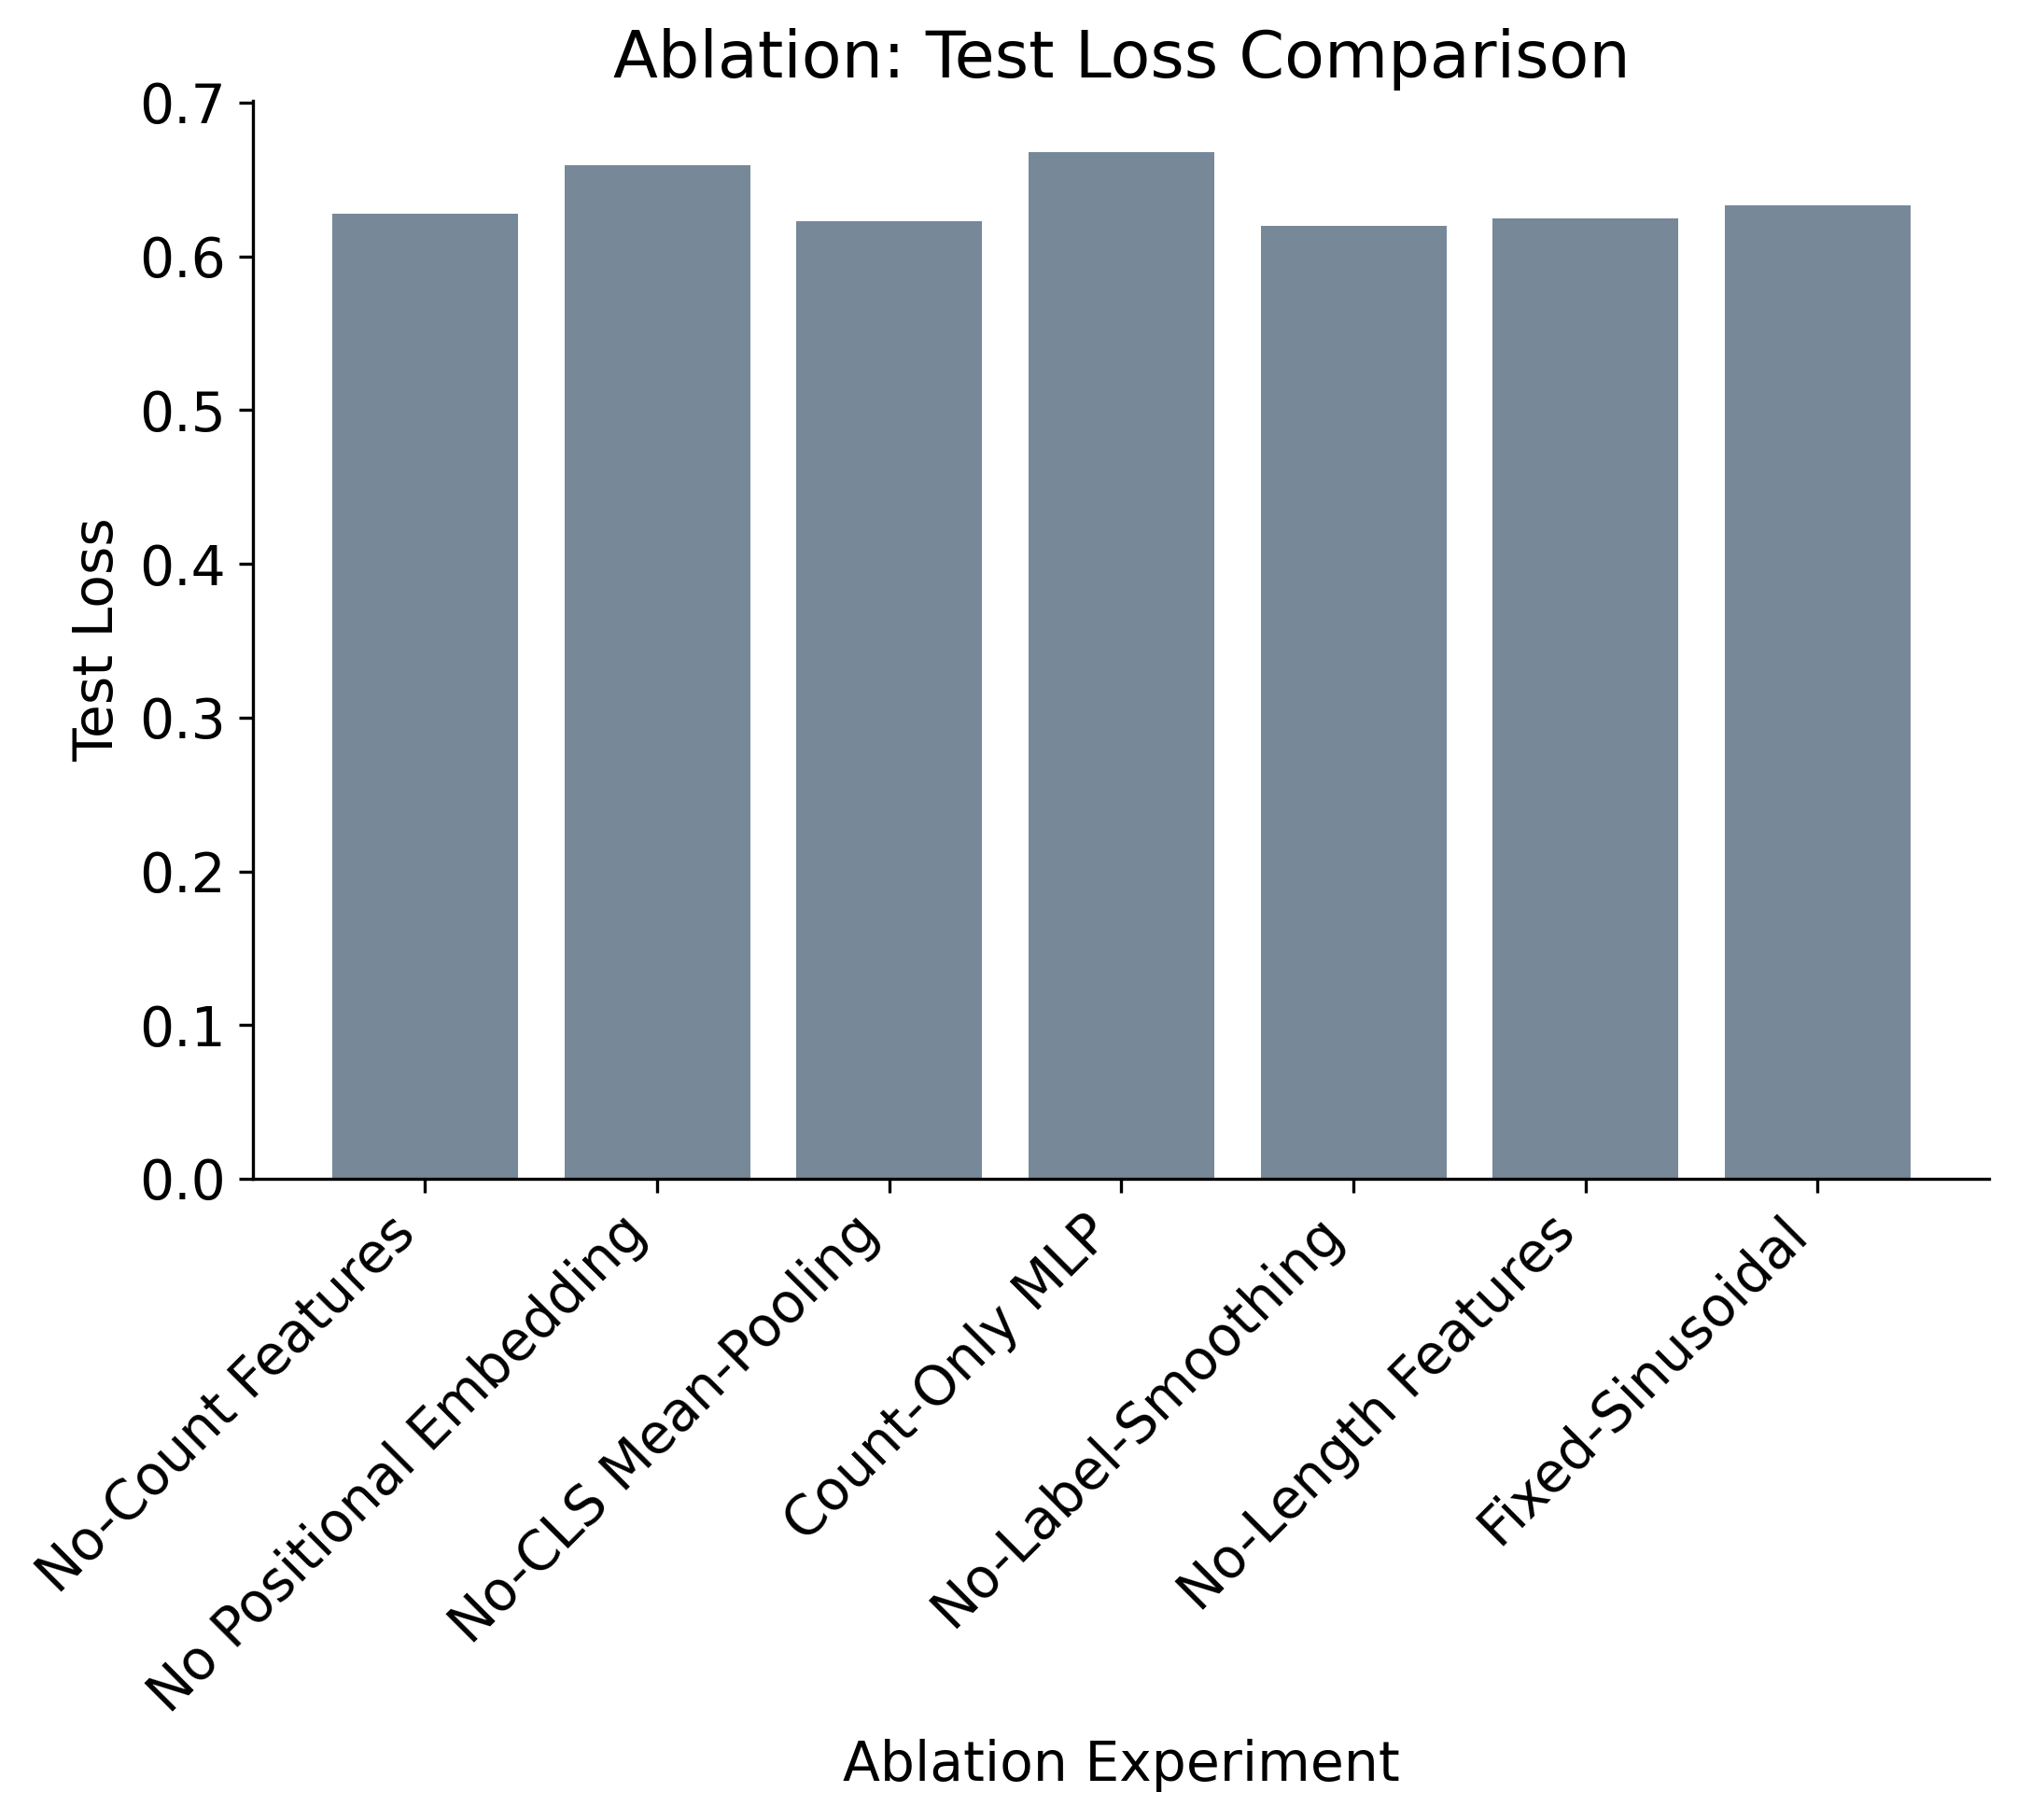
\includegraphics[width=0.8\textwidth]{Ablation_Test_Loss.png}\\
\vspace{1em}
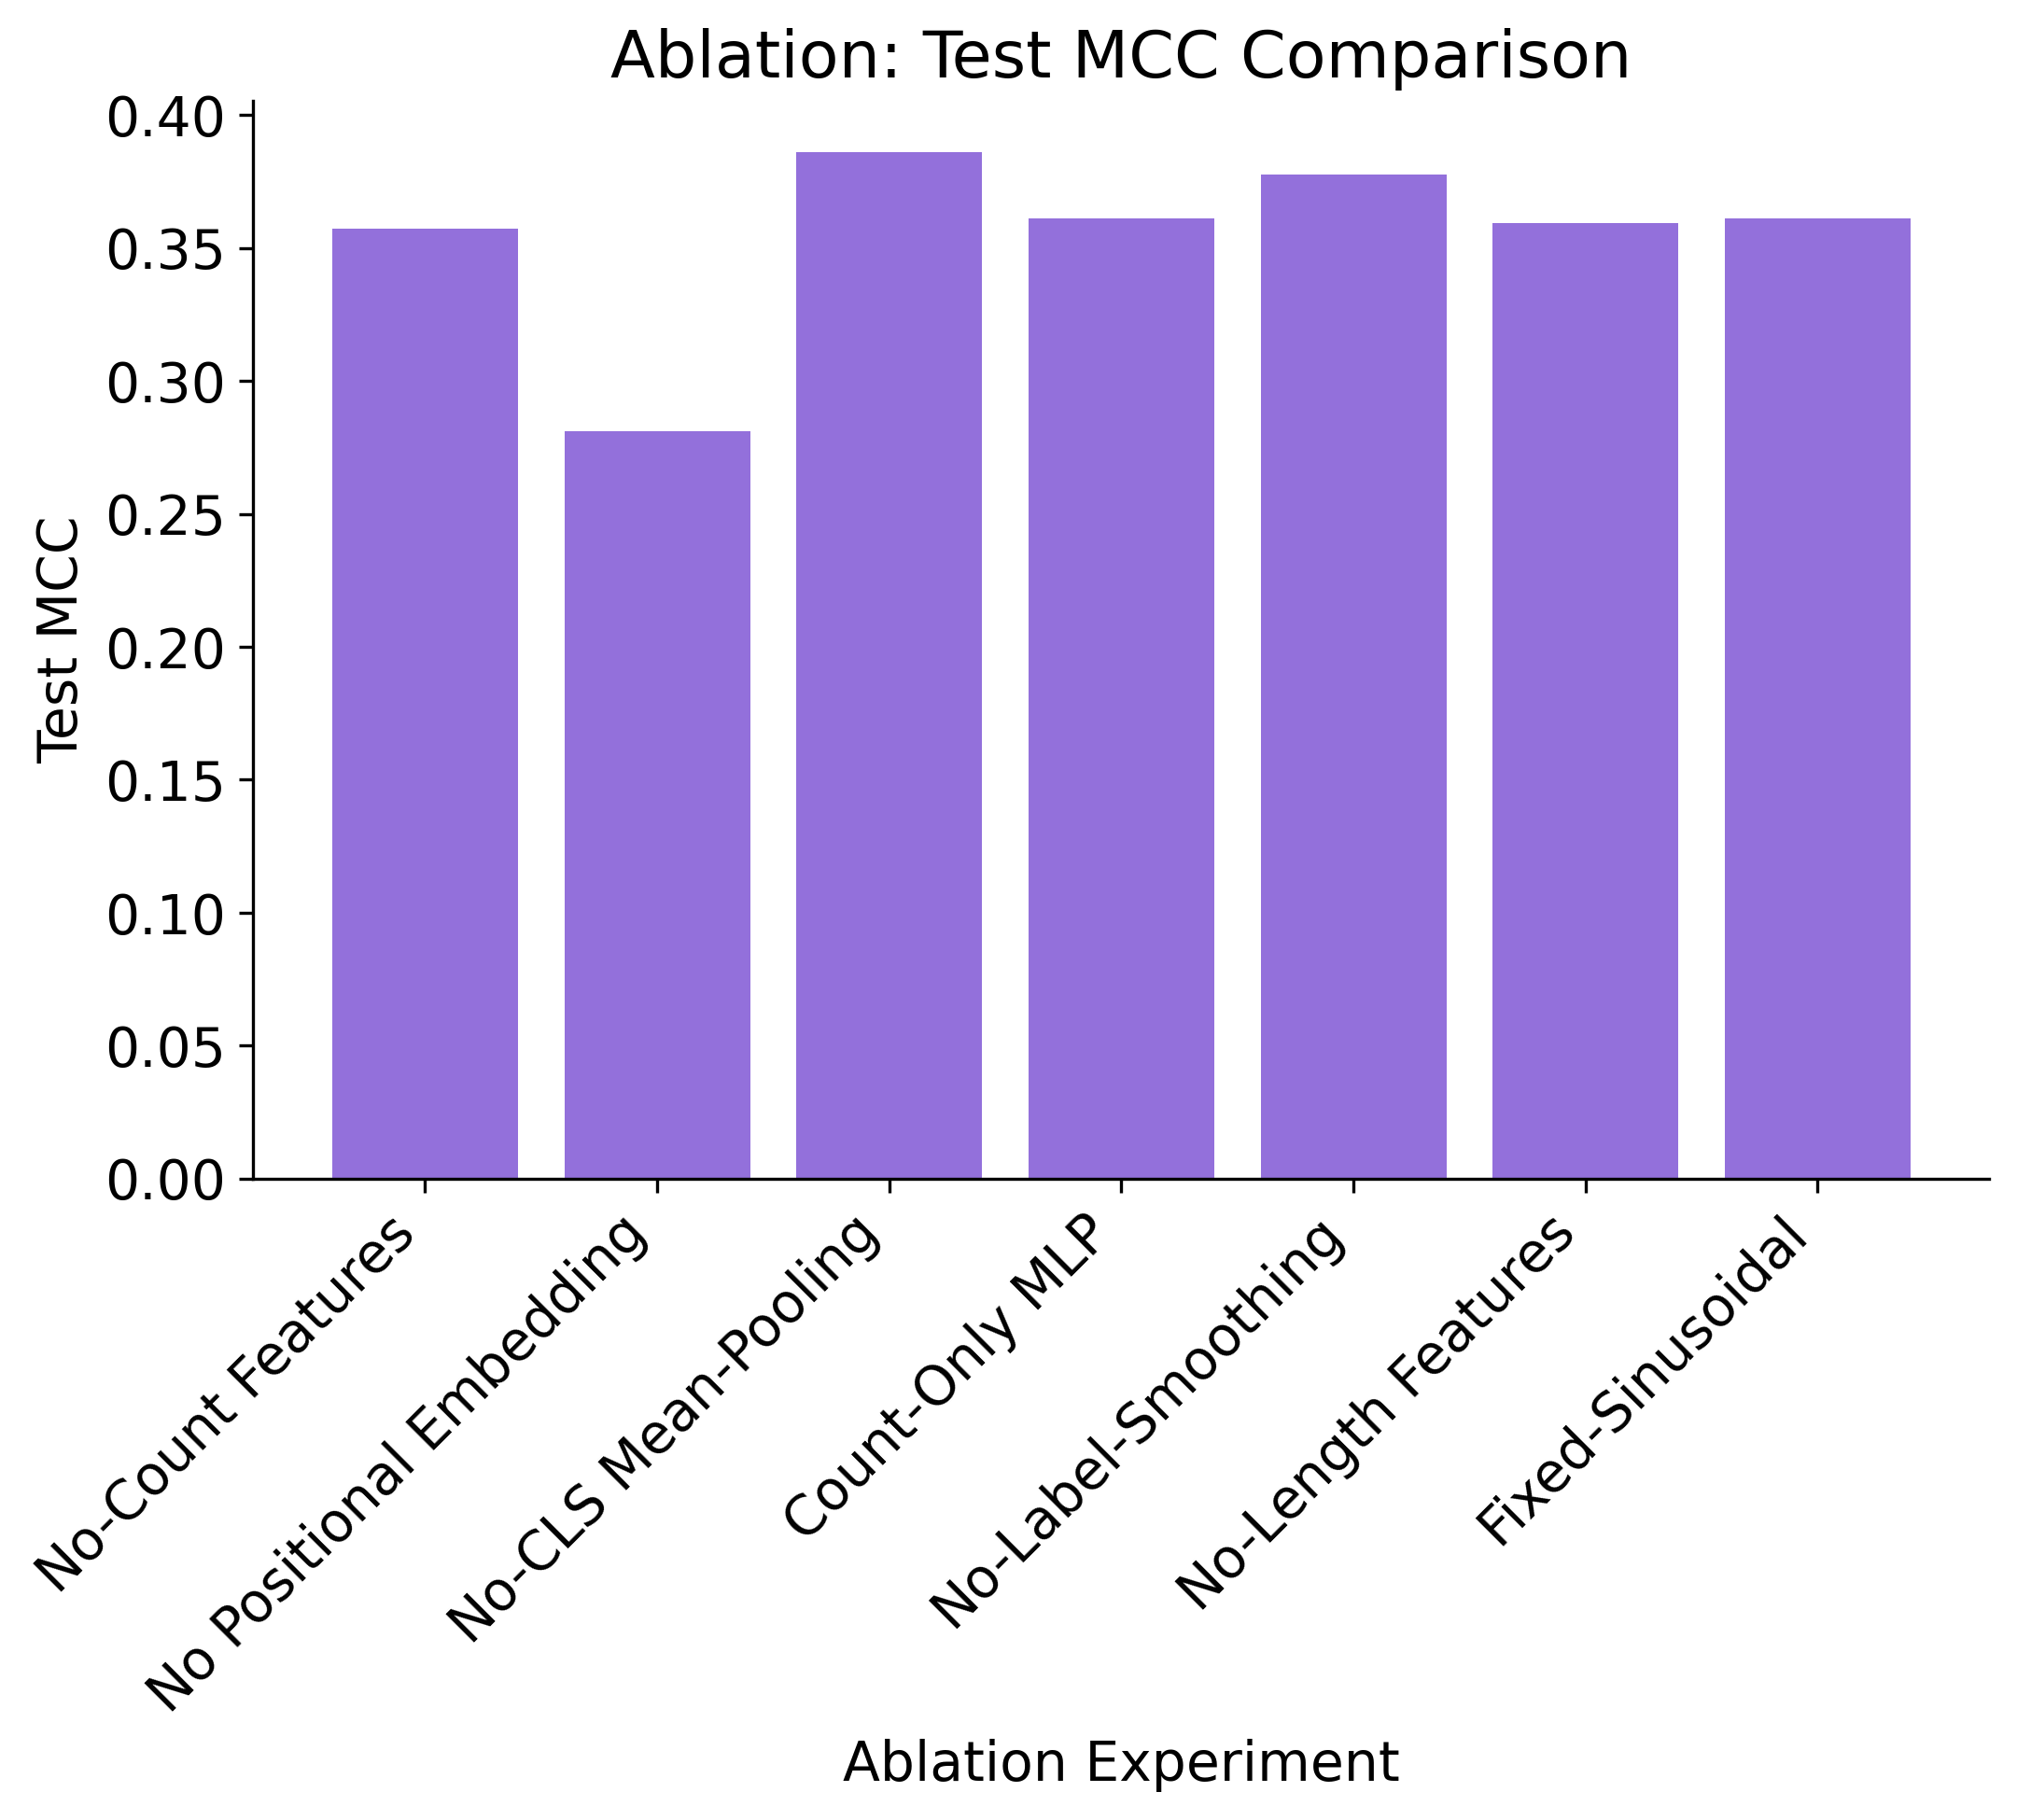
\includegraphics[width=0.8\textwidth]{Ablation_Test_MCC.png}\\
\vspace{1em}
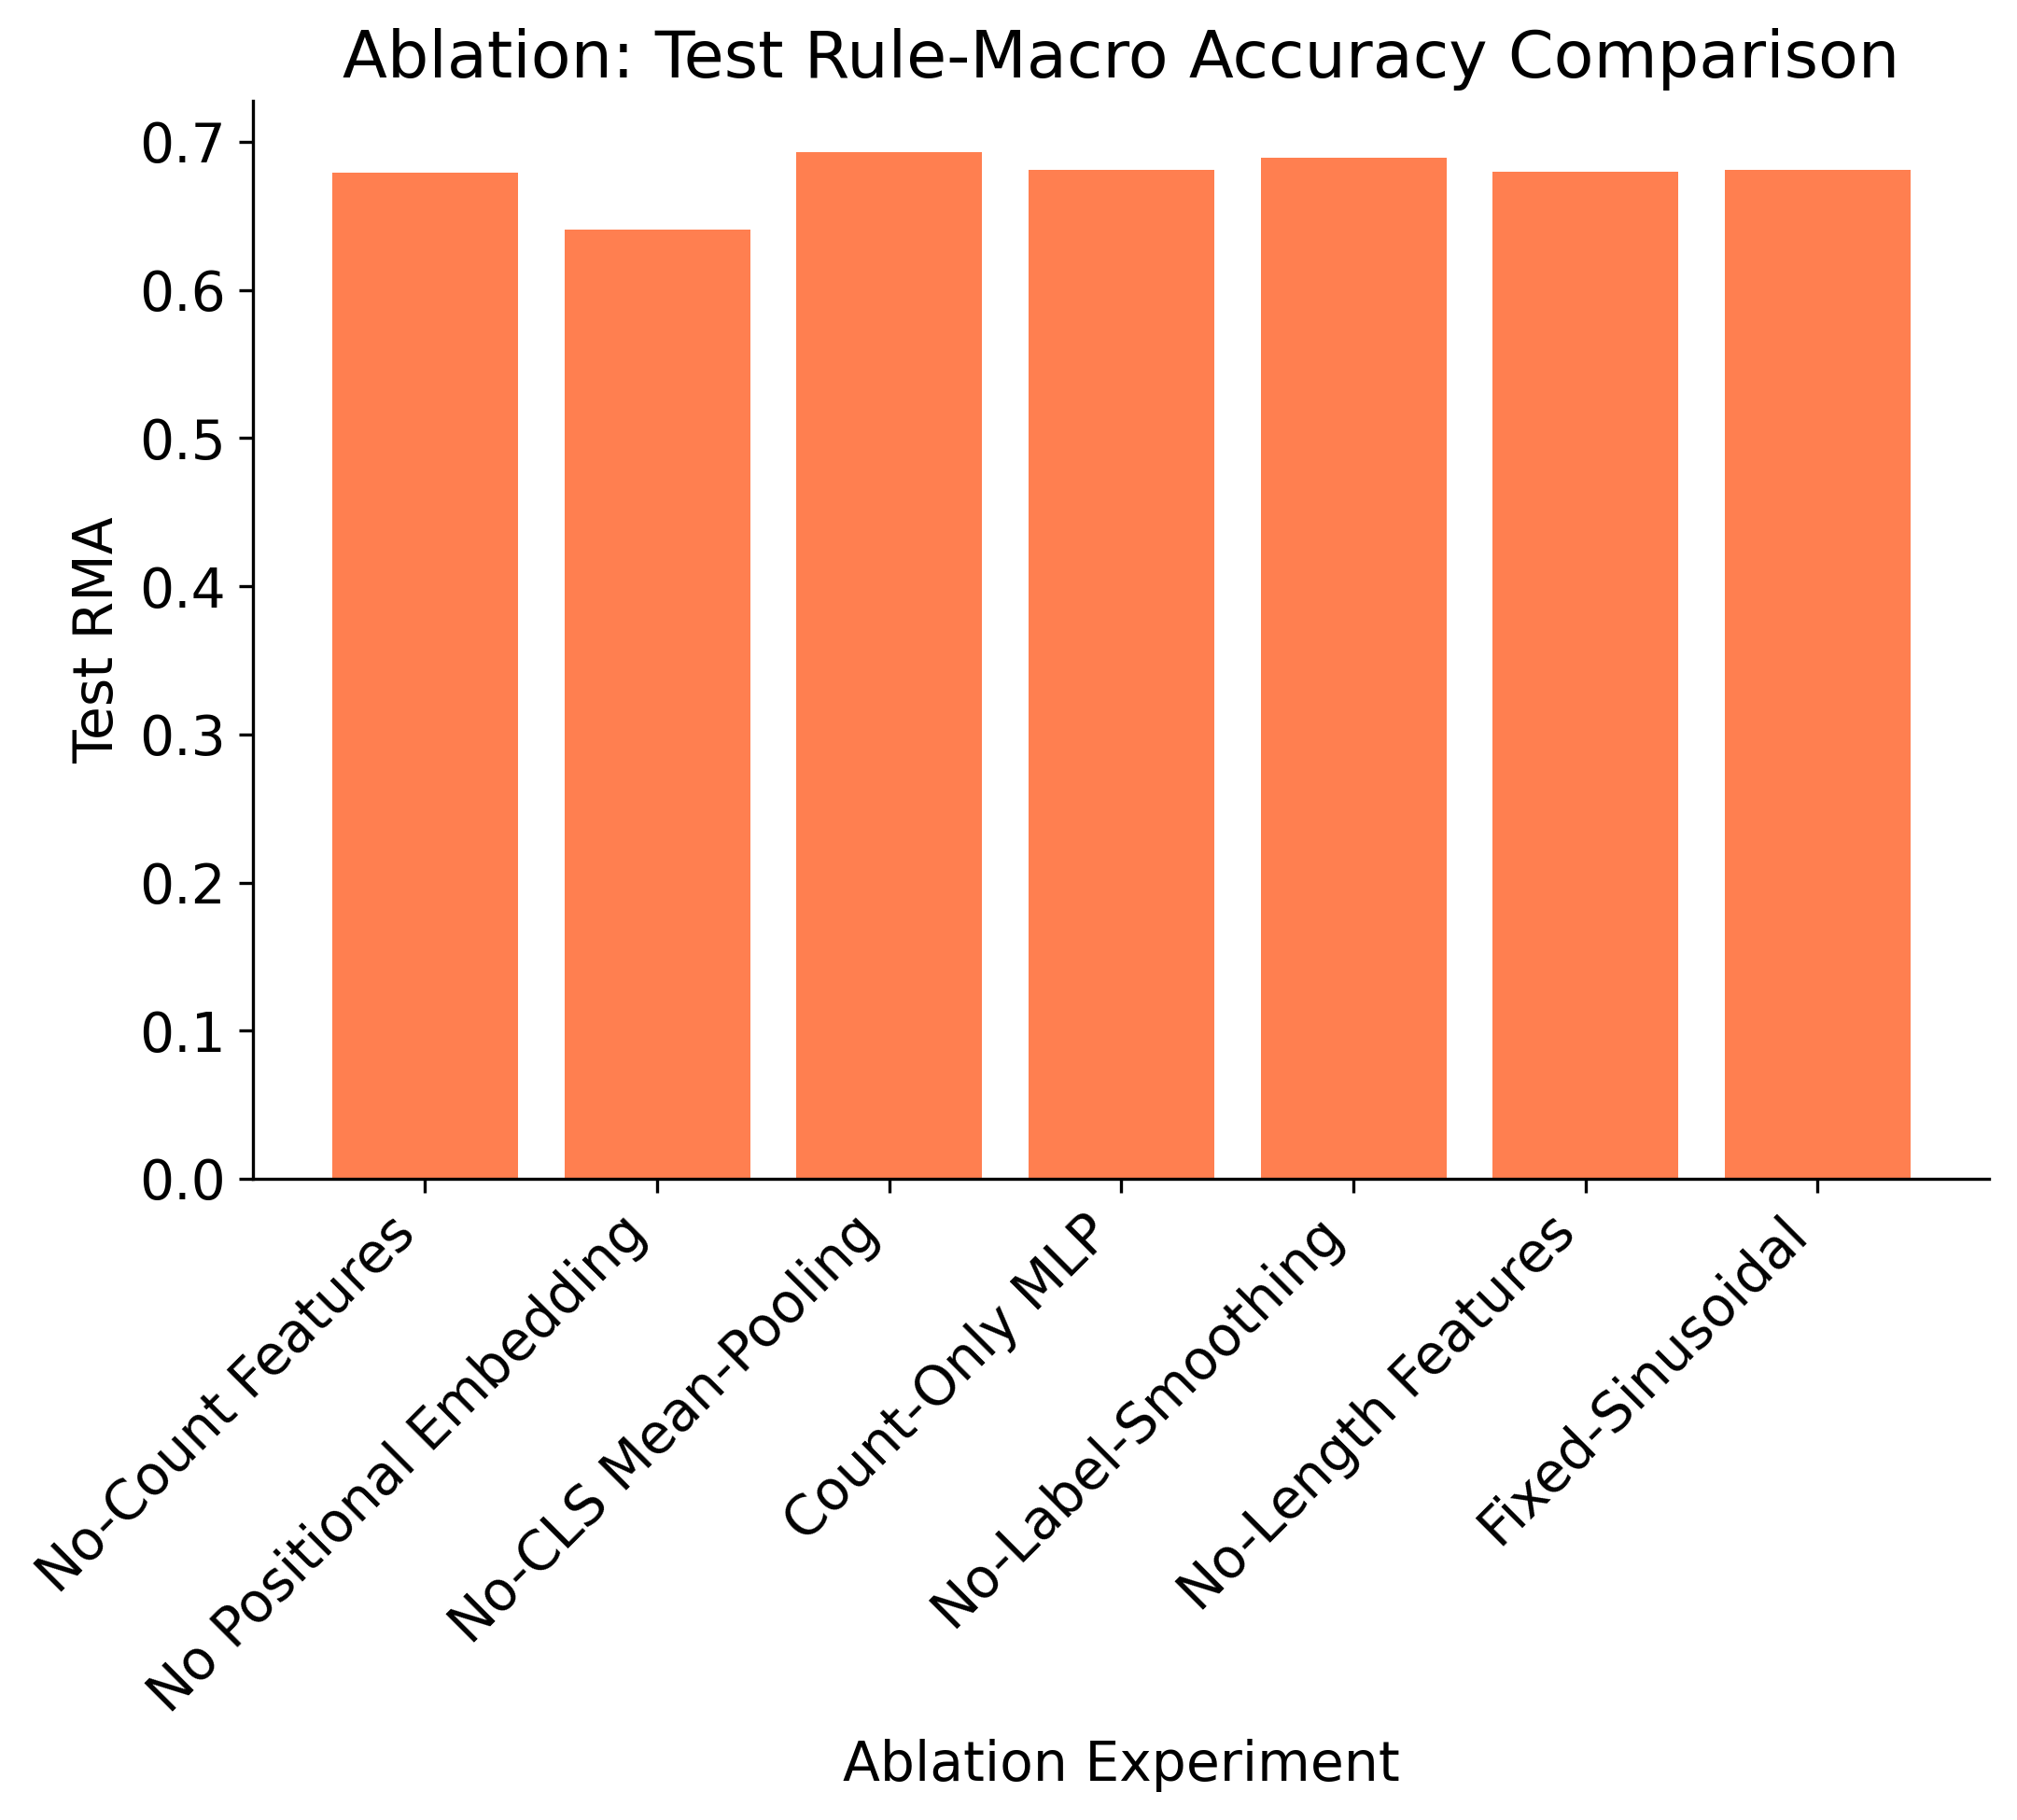
\includegraphics[width=0.8\textwidth]{Ablation_Test_RMA.png}
\caption{Ablation tests: accuracy, loss, MCC, and misclassification across ablation variants.}
\label{fig:ablation_multi}
\end{figure}

\end{document}